\documentclass[10pt,aspectratio=43]{beamer}

%% Fonts
\usepackage{multicol}
\usepackage{mathabx}
\usepackage[scaled]{helvet}
\usepackage{lmodern}
\usepackage{eulervm}
\usepackage{natbib}
\usepackage{booktabs}
\usepackage{amsfonts}
%\usepackage{multicol}
%\usefonttheme[onlymath]{serif}
%\usefonttheme{professionalfonts}
\usefonttheme{structurebold}
\usepackage{bm}


%% Color & Theme
\definecolor{SUblue}{RGB}{0,0,180}
\usecolortheme[RGB={0,0,180}]{structure}
\usetheme{Boadilla}
\setbeamertemplate{navigation symbols}{}
\setbeamertemplate{itemize items}[circle]
\setbeamertemplate{enumerate items}[circle]
\setbeamerfont{title}{size=\large}
\setbeamerfont{frametitle}{size=\large}
\setbeamerfont{framesubtitle}{size=\large,shape =$\color{violet}{\looparrowdownright}~$}
\setbeamercolor{title}{fg=white, bg= SUblue!75!green}
\setbeamercolor{framesubtitle}{fg=violet}
%% \setlength{\leftmargini}{5pt}

\hypersetup{
  colorlinks=true,
  linkcolor=blue,
  citecolor=blue,
  urlcolor=magenta}


\title[Feature-based time series forecasting]{\textbf{Time series forecasting based on
    \\automatic feature extraction}}

\author[Feng Li]{\includegraphics[height=2cm]{cufelogo}\\
  \vspace{0.5cm}\textbf{Feng Li}}

\institute[\url{http://feng.li/}]{\footnotesize{\textbf{School of Statistics and
      Mathematics\\ Central University of Finance and Economics}}}
\date{}

\begin{document}
%% Title page
\begin{frame}[plain]
  \addtocounter{framenumber}{-1}
  \titlepage

  \begin{itemize}
    \item \color{blue} \footnotesize{Joint with Yanfei Kang and Xixi Li}.
    \item \color{blue} \footnotesize{Feng Li's research is supported by
      National Natural Science Foundation of China}.
  \end{itemize}

\end{frame}

\section*{Outline}
\begin{frame}
  \frametitle{Outline}
  \addtocounter{framenumber}{-1}
\tableofcontents
\end{frame}

\section{Feature-based time series forecasting}




\begin{frame}{Motivation}

  \begin{itemize}
  \item Train a time series model (\emph{machine learning with dependent data}) is usually
    costly.

  \item New algorithms are developed every day.

  \centerline{\includegraphics[height=0.3\textheight]{figures/motivation}}

  \item Is there an efficient way to \textbf{forecast which algorithm works the best} for
    a particular time series?

  \end{itemize}


\end{frame}


\begin{frame}{Literature}

  \begin{itemize}
  \item Features of time series \(\rightarrow\) benefits in producing more accurate
    forecasting accuracies \citep{adam1973individual}.

  \item Features \(\rightarrow\) forecasting method selection rules
    \citep{meade2000evidence}.

  \item ``Horses for courses'' \(\rightarrow\) effects of time series features to the
    forecasting performances \citep{Petropoulos2014}.

  \item We could visualize the performances of different forecasting methods in a 2D space
    \(\rightarrow\) to get better understanding of their relative performances
    \citep{kang2017visualising}.

  \end{itemize}

\end{frame}

\begin{frame}{Traditional time series features}

  Transform a given time series \(\{x_1, x_2, \cdots, x_n\}\) to a feature
  vector \(F = (F_1, F_2, \cdots, F_p)'\) \citep{kang2017visualising,cikm2015}

  \begin{block}{A feature \(F_k\) can be any kind of function computed
      from a time series:}

    \begin{enumerate}
    \item
      A simple mean
    \item
      The parameter of a fitted model
    \item
      Some statistic intended to highlight an attribute of the data
    \item
      \ldots{}
    \end{enumerate}

  \end{block}

\end{frame}

\begin{frame}{Which features should we use?}

  \begin{itemize}
  \item \textbf{Bad News}: There does not exist the best feature representation of a time series
    \citep{fulcher2018feature}.
  \item
    Depends on both the \textbf{nature} of the time series being analysed,
    and the \textbf{purpose} of the analysis.

    \begin{itemize}
    \item
      With unit roots, the mean is not a meaningful feature without some
      constraints on the initial values.
    \item
      CPU usage every minute for a large number of servers: we observe a
      daily seasonality. The mean may provide useful comparative
      information despite the time series not being stationary.
    \end{itemize}
  \end{itemize}

\end{frame}

\begin{frame}
  \frametitle{Encoding time series to images}

  \begin{itemize}
  \item Let $R(i,j)$ be the element of the \textbf{time series image matrix} where $i$
    indexes time on the x-axis of the recurrence plot and $j$ indexes time on the y-axis;
  \item  \textbf{Recurrence Plot Encoding}
\begin{equation*}
  R(i, j) = \begin{cases}
    S, & if \parallel \overrightarrow{x(i)} -\overrightarrow{x(j)}\parallel/\epsilon>S,\\
    \parallel \overrightarrow{x(i)} -\overrightarrow{x(j)}\parallel/\epsilon, & otherwise,
  \end{cases}
\end{equation*}
  where $S$ is the threshold distance and $\epsilon$ is some small number.

\item \textbf{Gramian Angular Field Encoding} \citep{wang2015Imaging}: Given a time series
  $X={x_{1},x_{2},...,x_{n}}$ , we scale the series X into $[-1,~1]$.
\begin{equation*}
 { x } _ { i } = \frac { \left( x _ { i } - \max ( X ) + \left( x _ { i } - \min ( X ) \right) \right. } { \max ( X ) - \min ( X ) }
\end{equation*}
Then, we convert the scaled time series X into ``polar coordinates''.

  \end{itemize}

\end{frame}



\section{Encoding time series to images}

\begin{frame}
  \frametitle{Encoding time series to images}
  \framesubtitle{}


  \begin{figure}[thb]
    \centering
    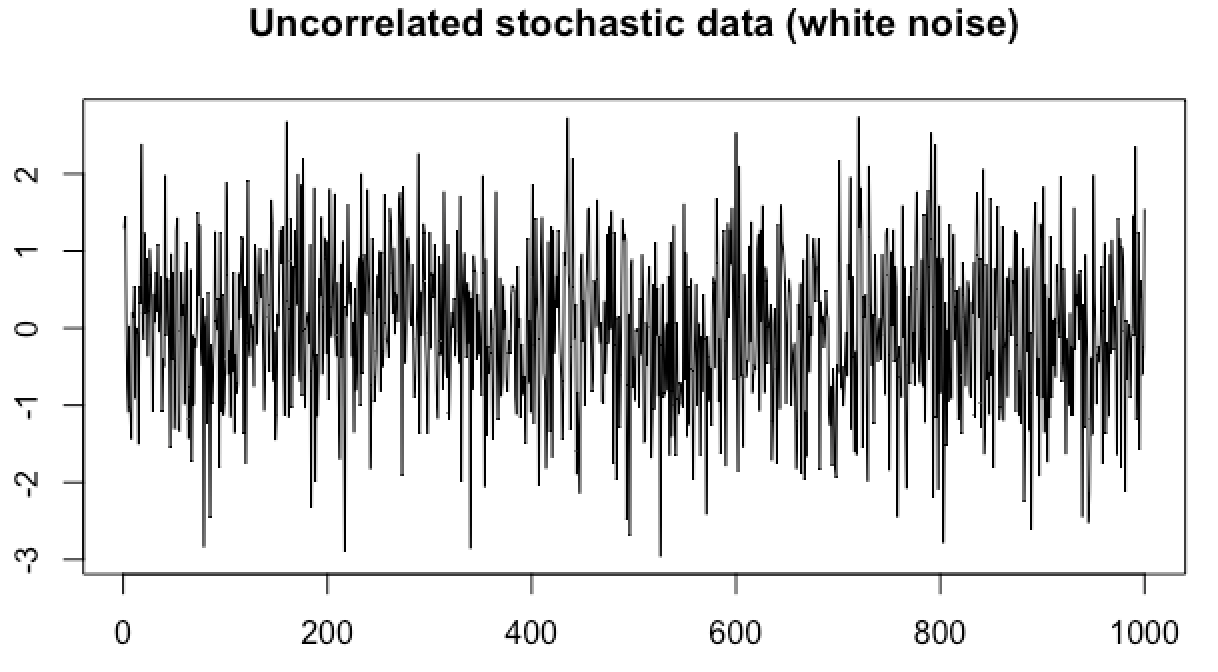
\includegraphics[width=0.25\linewidth]{figures/white_noise.png}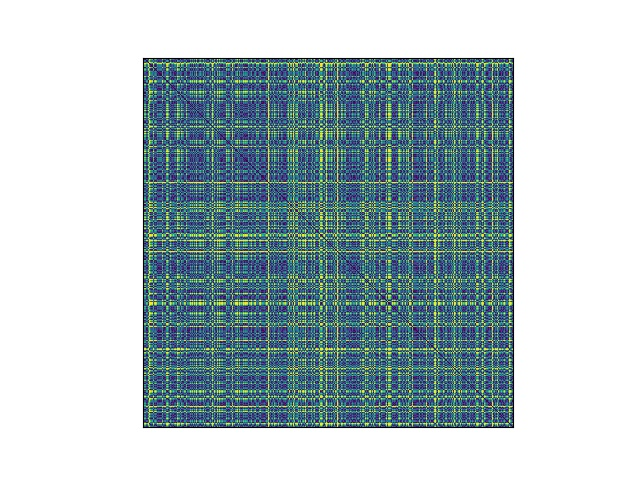
\includegraphics[width=0.25\linewidth]{figures/white_noise_R.jpg}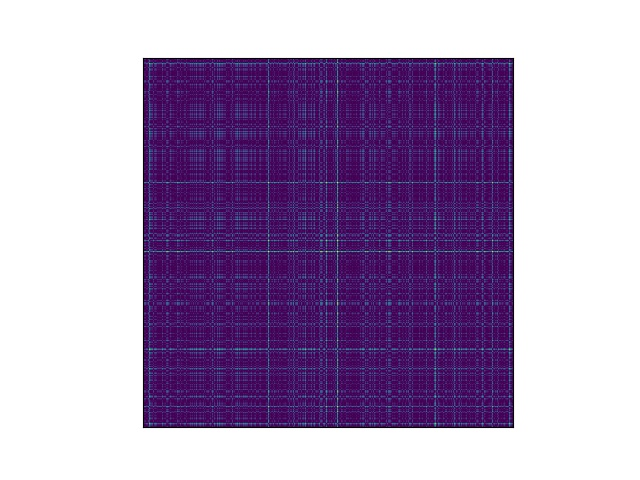
\includegraphics[width=0.25\linewidth]{figures/white_noise_GAF.jpg}\\
    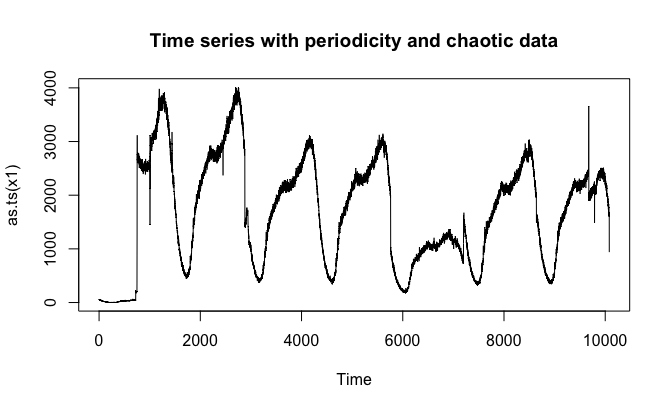
\includegraphics[width=0.25\linewidth]{figures/time_seires_with_frequency.png}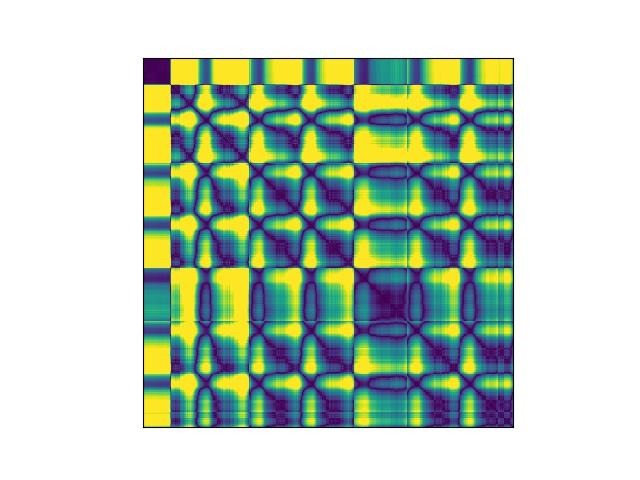
\includegraphics[width=0.25\linewidth]{figures/period_RP.jpg}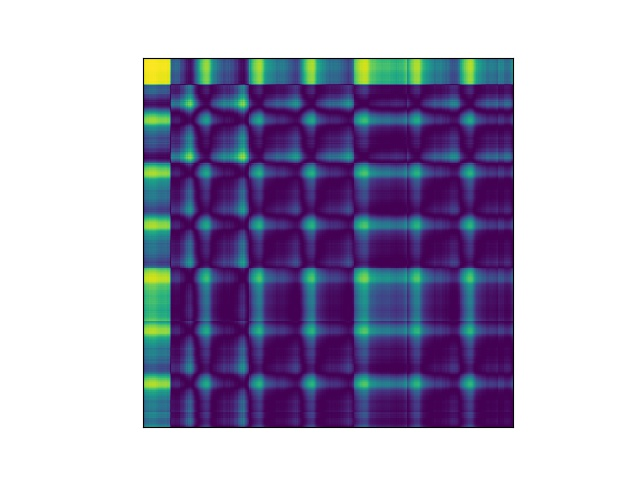
\includegraphics[width=0.25\linewidth]{figures/period_GAF.jpg}\\
    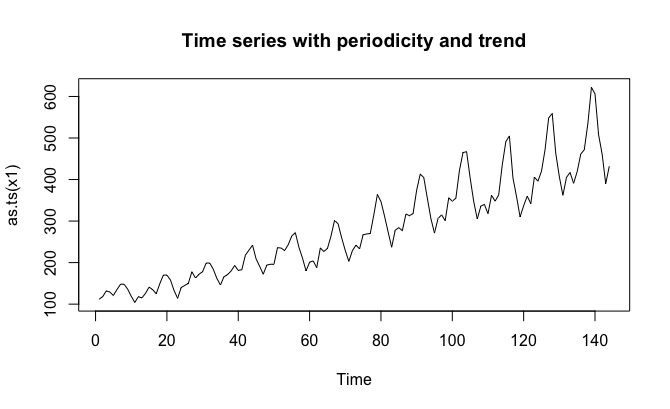
\includegraphics[width=0.25\linewidth]{figures/Period_data_with_linear_trend.png}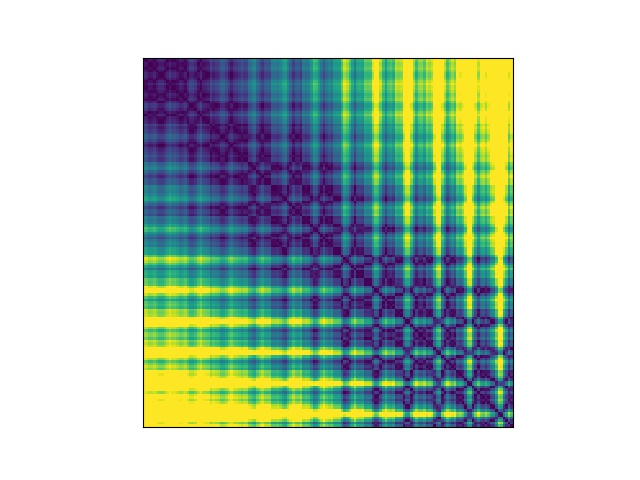
\includegraphics[width=0.25\linewidth]{figures/trend_period_RP.jpg}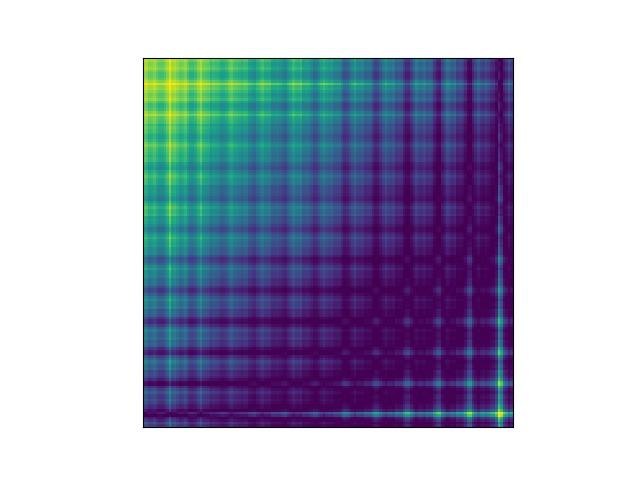
\includegraphics[width=0.25\linewidth]{figures/trend_period_GAF.jpg}\\
    \caption{Typical examples of recurrence plot(the second column) and Gramian Angular
      Field(the third column)}
  \label{fig:RP-egs}
\end{figure}

\end{frame}

\begin{frame}
  \frametitle{Image features}
  \begin{itemize}
  \item The original Bag of Features (BoF) model, which extracts features from one-dimensional
signal segments, has achieved a great success in time series classification
\citep{baydogan2013bag, wang2013bag}.
\item \citet{hatami2017bag} transform time-series into
two-dimensional recurrence images with recurrence plot \citep{eckmann1987recurrence} and
then applies the BoF model.

\item \citep{Razavian2014CNN} use the features acquired by the convolutional neural
  network as the input of the classifier, which significantly improves the accuracy of
  image classification.
  \end{itemize}
\end{frame}

\section{Image-based time series feature extraction}


\begin{frame}
  \frametitle{Image-based time series feature extraction}
  \framesubtitle{Scale-invariant feature transform (SIFT)}

  \begin{itemize}
  \item The scale space of an image is defined as the original image is convoluted with a
    variable-scale 2-dimensional Gaussian function.
  \item Key points are then taken as maxima/minima of the difference of Gaussians that occur at multiple scales.

  \item In our study, we use a 128-elements vector to characterize the key descriptors.
  \item Firstly, we establish an 8-direction histogram in each $4 \times 4$ sub-region, and a
    total of 16 sub-regions in the $16 \times 16$ region around the key point are
    calculated. Then we calculate the magnitude and direction of each pixel's gradient
    magnitude and add to the sub-region.
  \item In the end, a total of 128-dimensional image data based on histograms are
    generated.
  \item The sift method calculates the distribution characteristics of feature points in
    the whole image, and then generates a global histogram, so the spatial distribution
    information of the image is lost, and the image may not be accurately identified.

  \item A spatial pyramid method statistically distributes image feature points at
    different resolutions to obtain spatial information of images.
  \end{itemize}
\end{frame}

\begin{frame}
  \frametitle{Image-based time series feature extraction}
  \framesubtitle{Scale-invariant feature transform (SIFT)}

\begin{figure}
  \centering 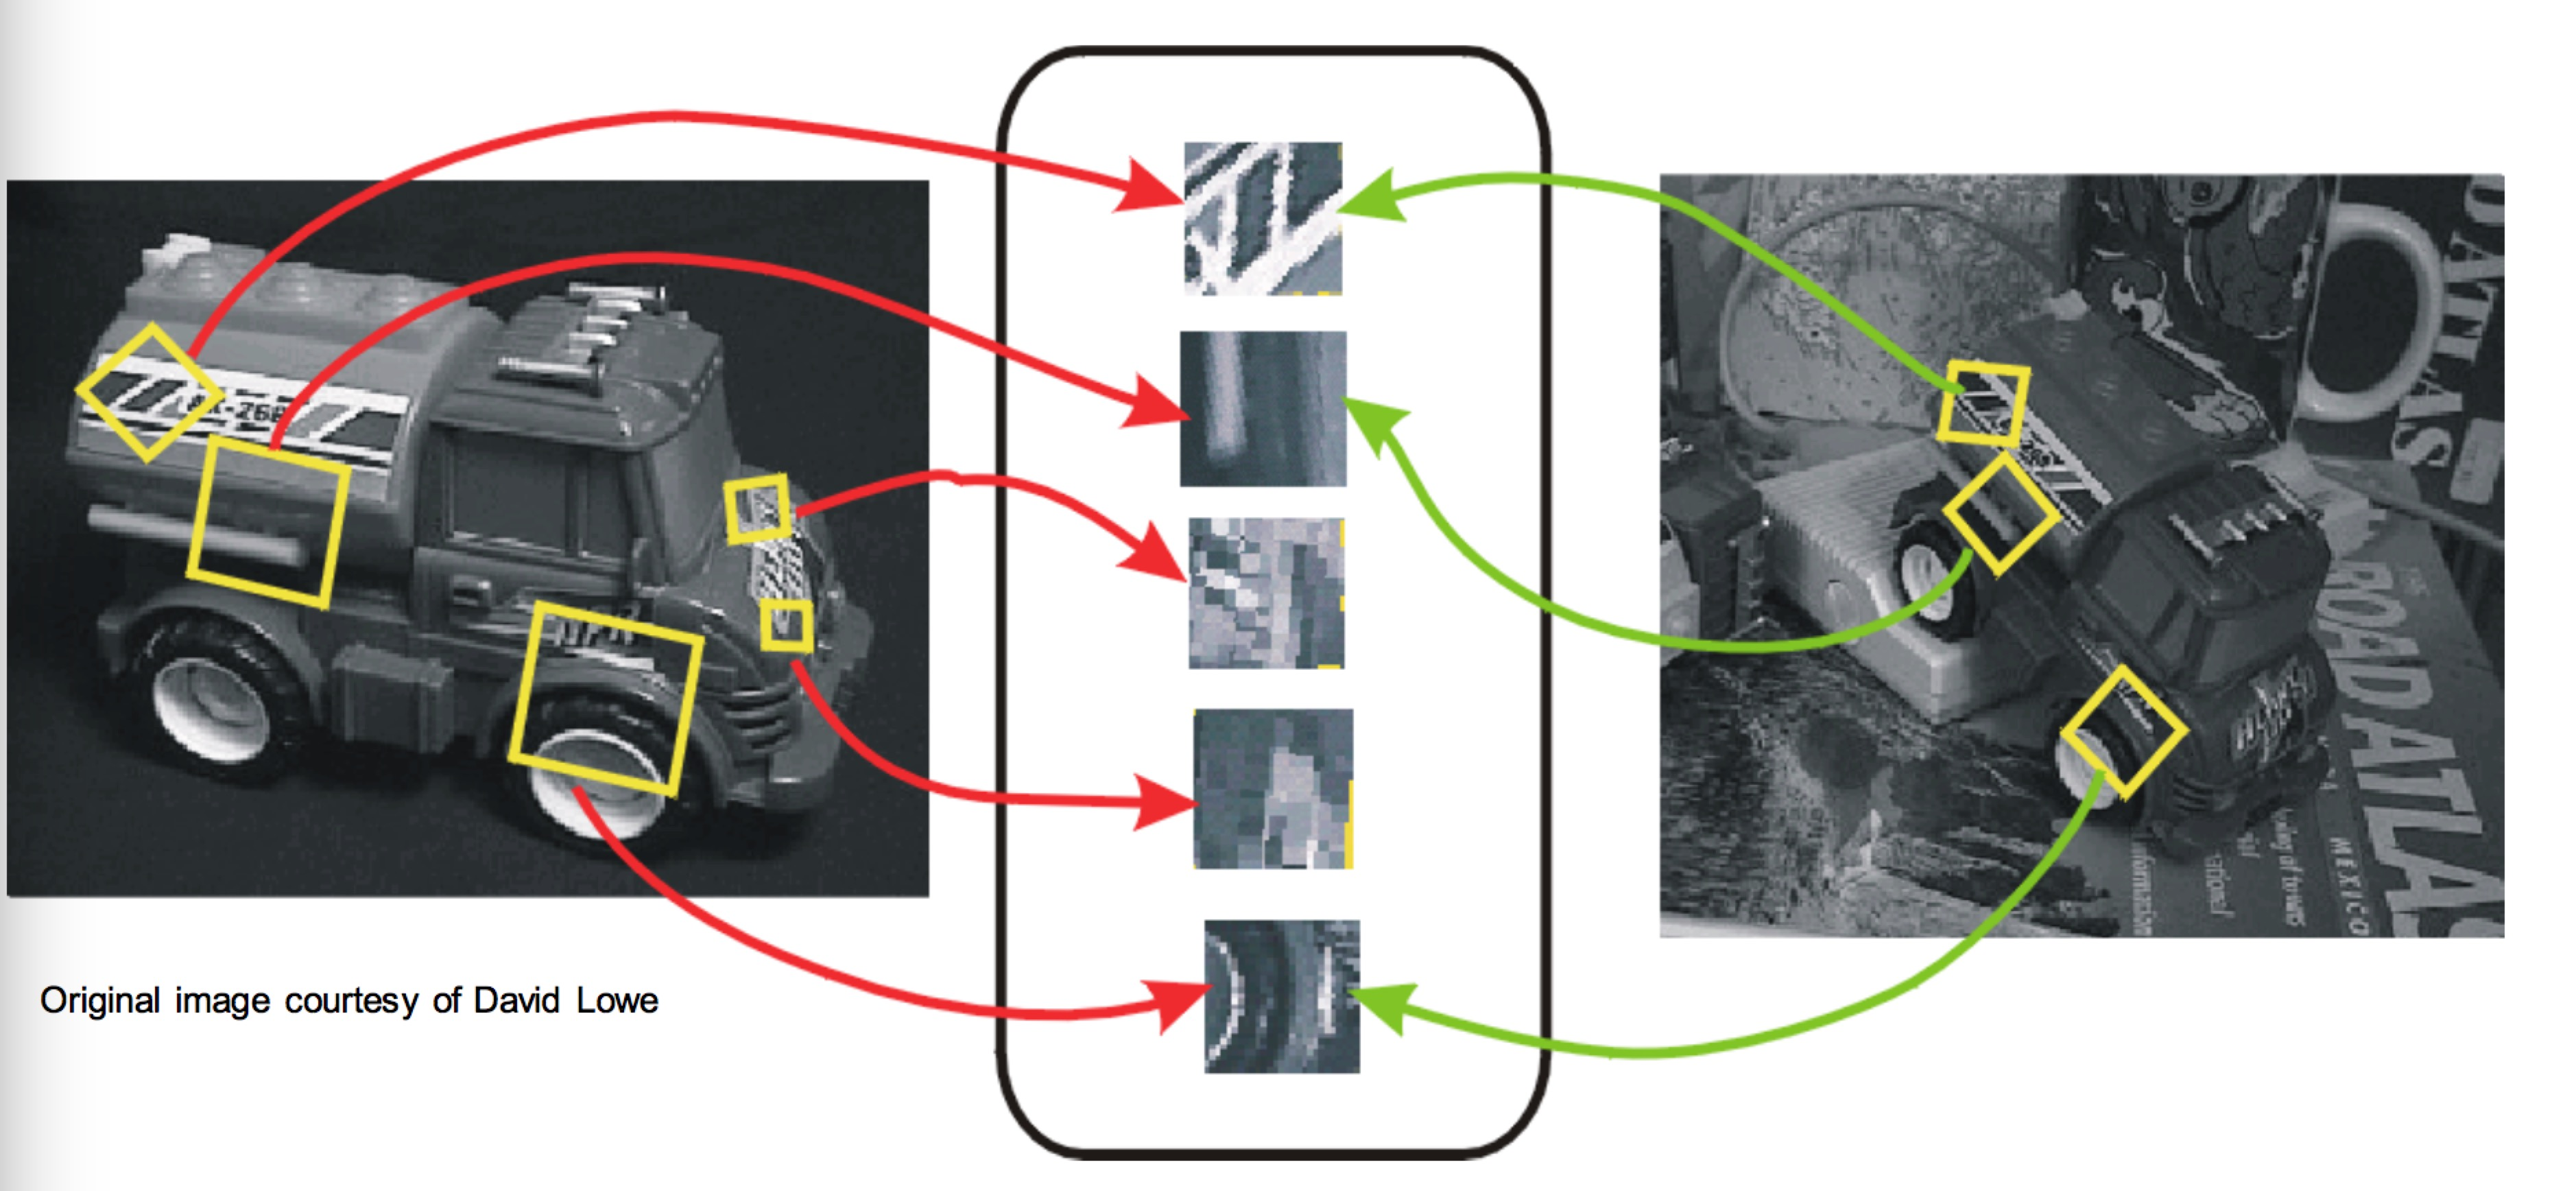
\includegraphics[width=1\linewidth]{figures/sift.png}
  \caption{Image feature extraction with scale-invariant feature transform}
  \label{fig:Feature extraction with SIFT}
\end{figure}

\end{frame}


\begin{frame}
  \frametitle{Image-based time series feature extraction}
  \framesubtitle{Scale-invariant feature transform (SIFT)}

\begin{figure}
  \centering 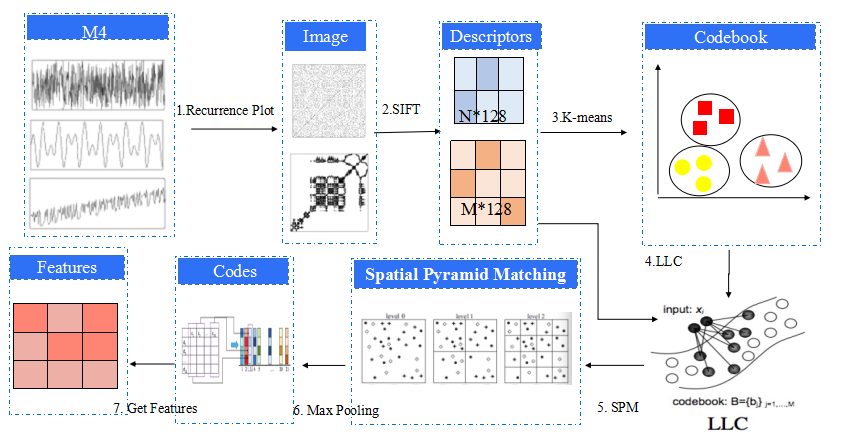
\includegraphics[width=1\linewidth]{figures/feature_extraction_sift.png}
  \caption{Image Feature Extraction with scale-invariant feature transform}
  \label{fig:Feature extraction with traditional image processing method}
\end{figure}

\end{frame}

\begin{frame}
  \frametitle{Image-based time series feature extraction}
  \framesubtitle{Transfer learning with fine-tuning}

  \begin{itemize}
  \item The deep convolutional neural networks has greater advantages in accuracy compared
    with the traditional image features.

  \item But building models from scratch is complex and time consuming.


  \item One could used a pretrained trained neural network model and make adjustments to
    her own task -- \textbf{Transfer learning}.

  \end{itemize}
\end{frame}


\begin{frame}
  \frametitle{Image-based time series feature extraction}
  \framesubtitle{Transfer learning with fine-tuning}

\begin{figure}[thb]
  \centering
  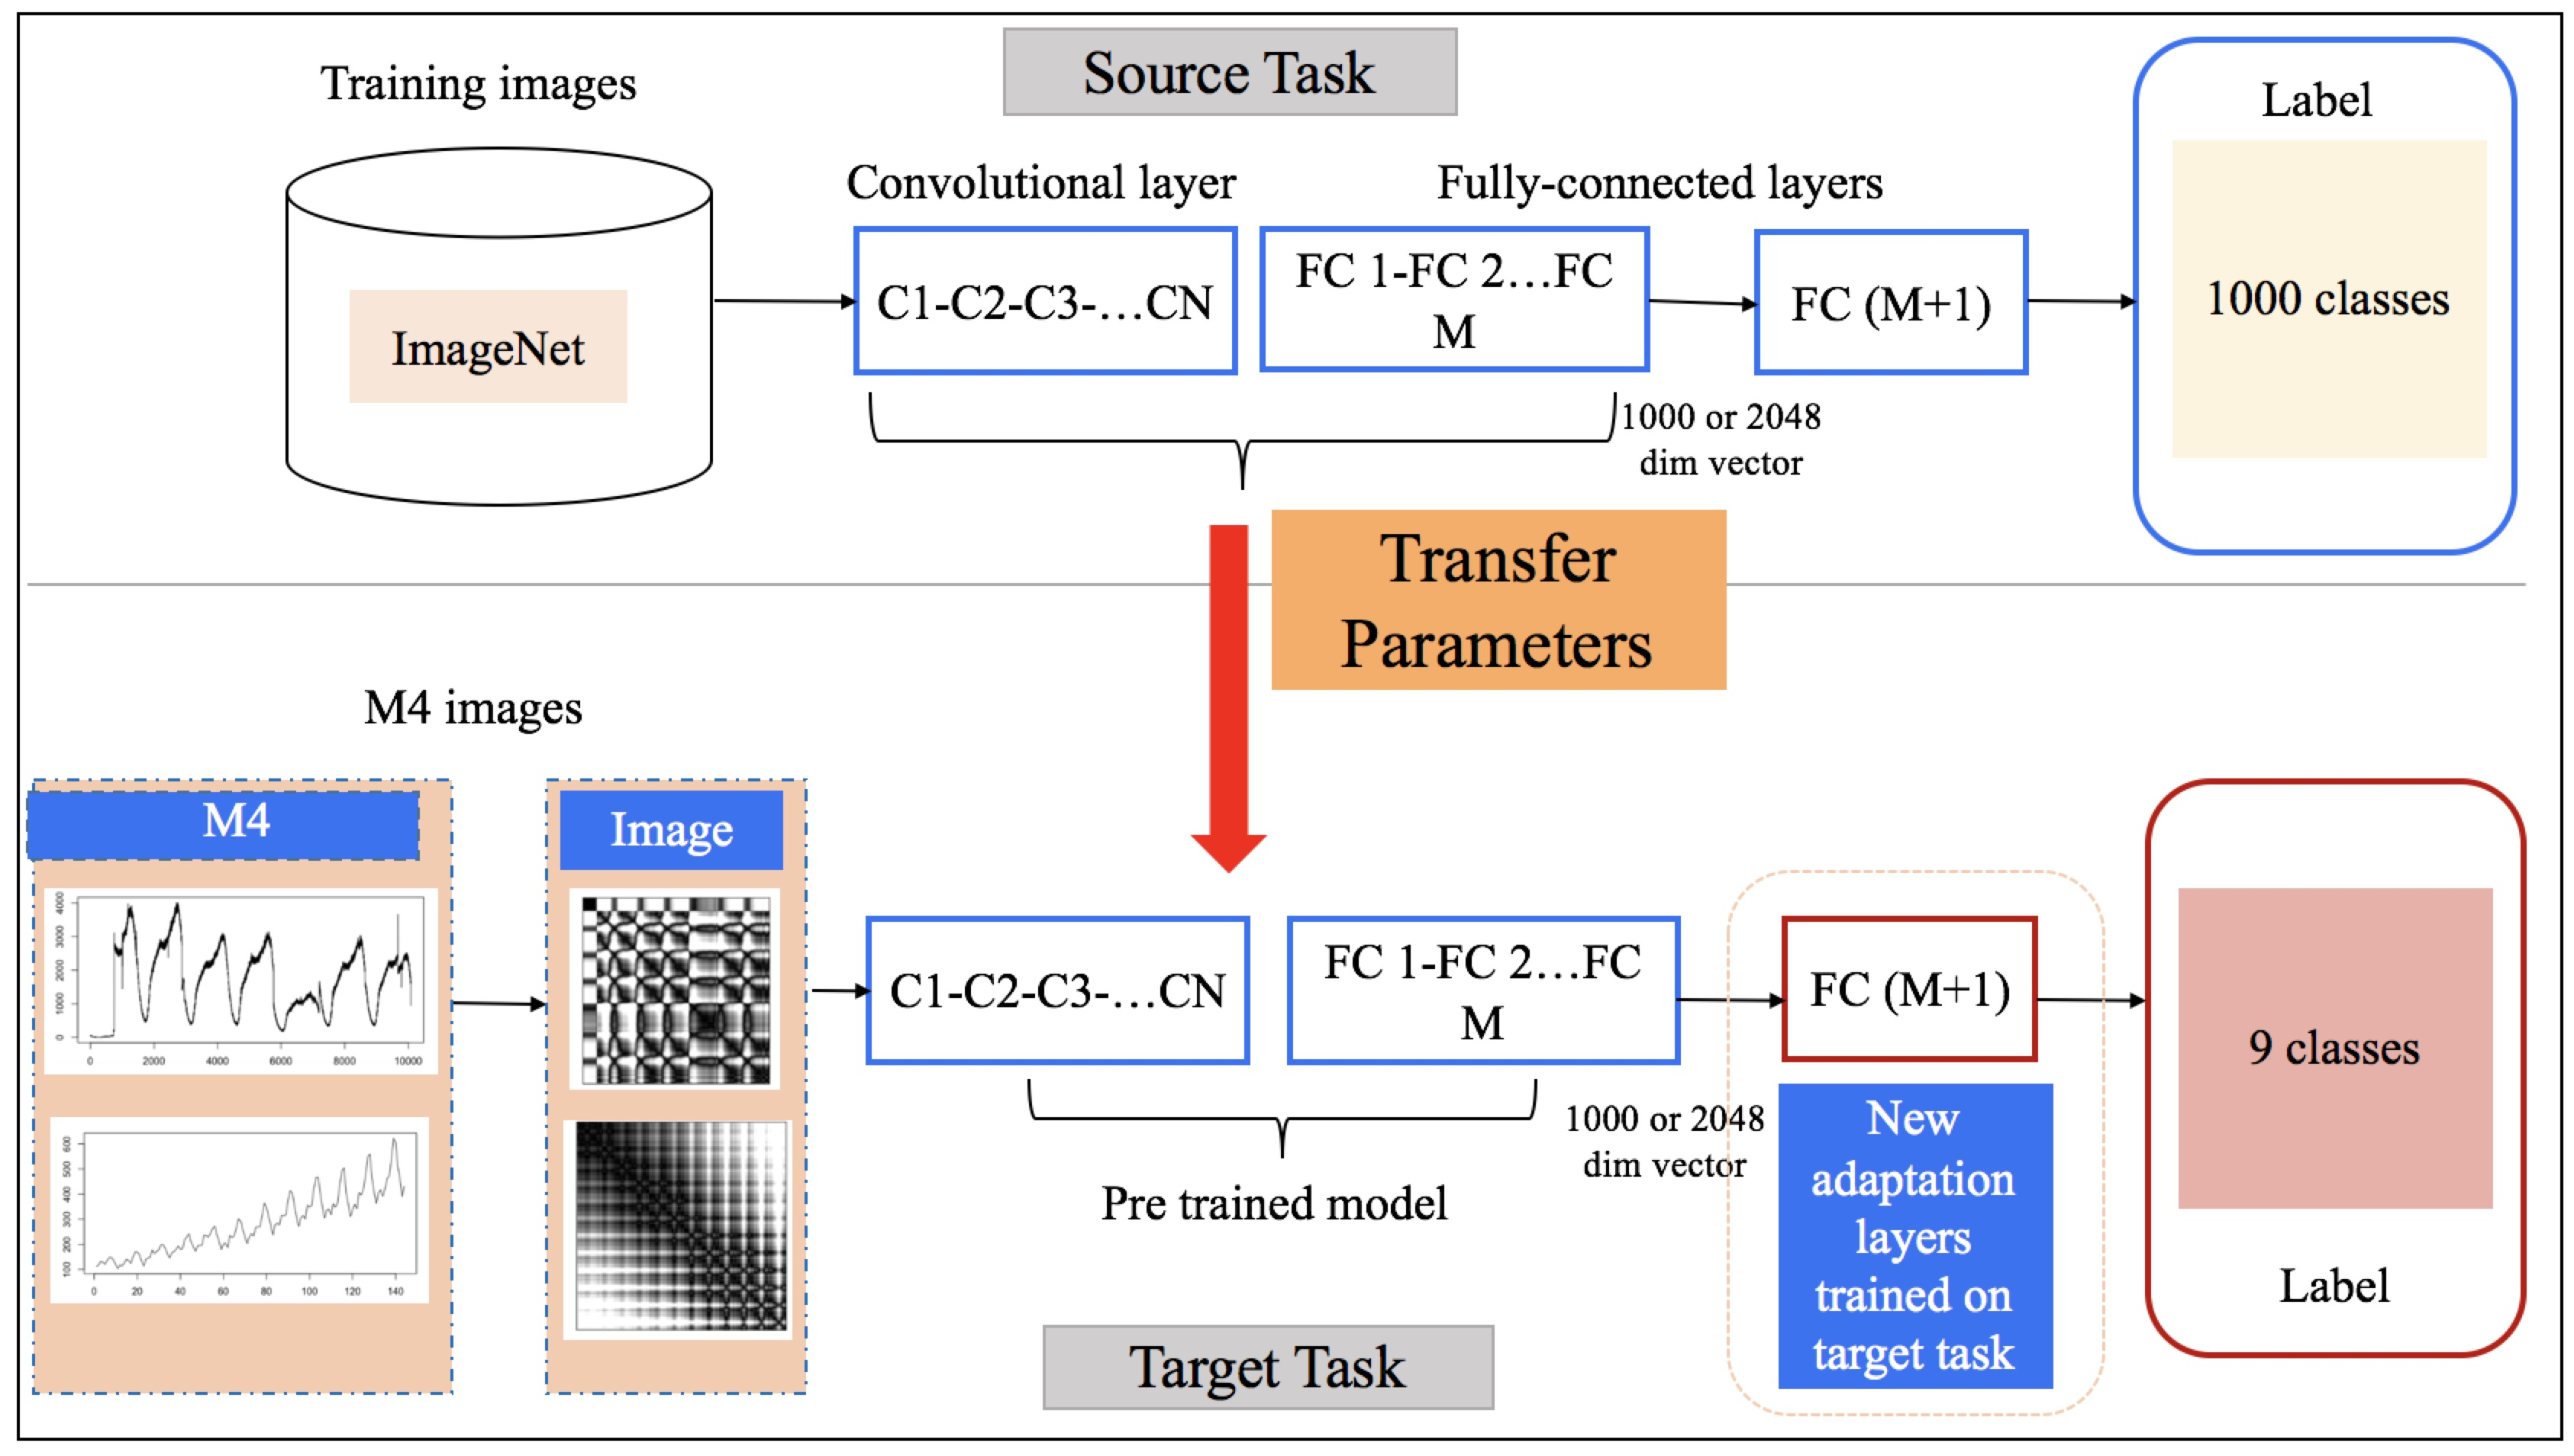
\includegraphics[width=0.8\linewidth]{figures/transfer-learning.jpg}
  \caption{\footnotesize{Transfer Learning-Fine-Tuning. We can train the Inception\citep{Szegedy2016Rethinking}, ResNet\citep{Szegedy2016Inception}, VGG\citep{Simonyan2014Very} and other classic CNN models with large dataset ImageNet\citep{Deng2009ImageNet}. With the pre trained model, we fix the parameters of the previous layers, and fine-tune the next few layers for our task. In this way, the speed of network training will be greatly accelerated, and it will also greatly promote the performance of our task.}}
  \label{fig:transfer-learning}
\end{figure}
\end{frame}

\begin{frame}
  \frametitle{Time series forecasting methods}

  \begin{itemize}
\item \textbf{Naive}: uses the most recent observation as the forecast for all future periods.

\item \textbf{Seasonal naive}: forecasts are equal to the most recent observation from the
  corresponding time of year.

\item \textbf{The Theta method}: It performed particularly well in the M3-Competition proposed by
  \citet{Assimakopoulos2000The}.

\item \textbf{ETS}: exponential smoothing state space modeling, which is used widely as a general
  forecasting algorithm for trended and seasonal time series proposed by
  \citet{Hyndman2017A}.

\item \textbf{ARIMA}: autoregressive integrated moving average models, as implemented in the
  automated algorithm by \citet{HK08}.

\item \textbf{STL-AR}: an AR model is fitted to the seasonally adjusted series obtained from a STL
  decomposition proposed by \citet{cleveland1990stl}.

\item \textbf{Nnetar}: It fits a neural network model to a time series with lagged values of the
  time series as inputs (and possibly some other exogenous inputs).

\item \textbf{Rw-drift}: Random Walk with Drift.

\item \textbf{Tbats}: A Tbats model differs from dynamic harmonic regression in that the
  seasonality is allowed to change slowly over time in a Tbats model, while harmonic
  regression terms force the seasonal patterns to repeat periodically without changing, as
  implemented in the automated algorithm by \citet{HK08}.
\end{itemize}
\end{frame}

\section{Model selection and averaging}


\begin{frame}
  \frametitle{Forecast loss measurement}
  \begin{itemize}
  \item \textbf{Forecast loss measurement}: Overall Weighted Average (OWA) is an indicator
    of two accuracy measures: the Mean Absolute Scaled Error (MASE) and the symmetric Mean
    Absolute Percentage (sMAPE).

\begin{equation*}
  \begin{aligned}
    \mathrm{sMAPE}&=\frac{1}{h}\sum_{t=1}^h\frac{2\mid Y_{t}-\widehat{Y_{t}}\mid}{\mid Y_{t}\mid+\mid\widehat{Y_{t}} \mid},\\
    \mathrm{MASE}&=\frac{1}{h}\frac{\sum_{t=1}^h\mid Y_{t}-\widehat{Y_{t}} \mid}{\frac{1}{n-m}\sum_{t=m+1}^n\mid Y_{t}-Y_{t-m} \mid},\\
    \mathrm{OWA}&=\frac{\mathrm{sMAPE /sMPAE + MASE/MASE}}{2},
  \end{aligned}
\end{equation*}



\item Train a high dimensional regression model (Lasso) with $X_{train}$ and $M ASE$
\item Calculate predicted $MASE$ with $X_{test}$ using $R_i$
\end{itemize}

\end{frame}

\begin{frame}
  \frametitle{Model selection}

\begin{figure}[htb]
  \centering
  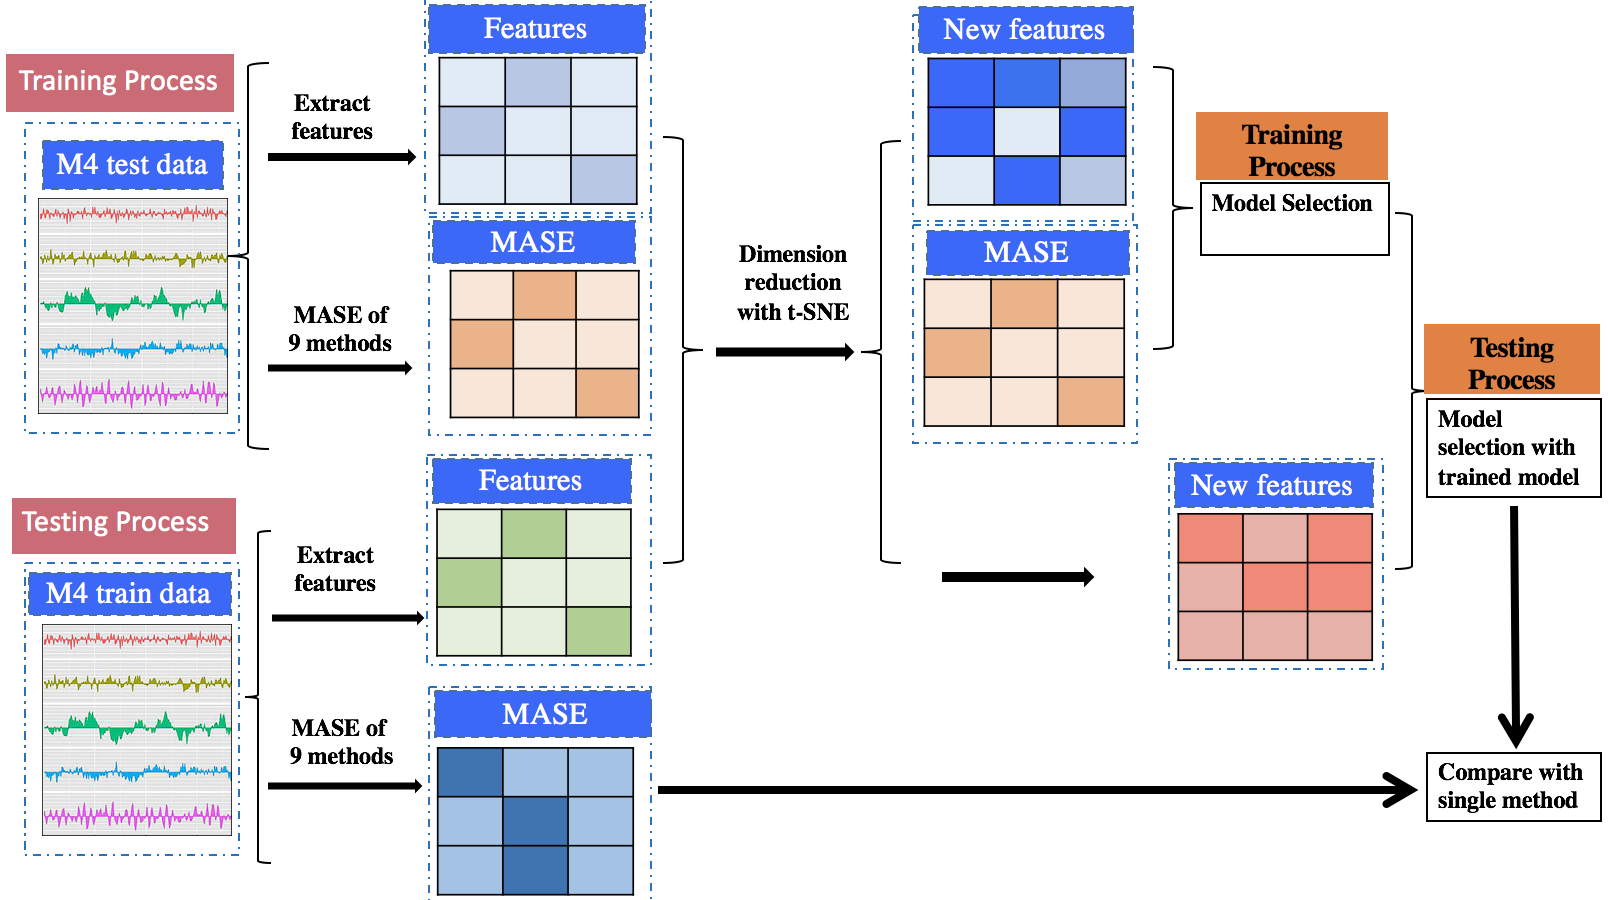
\includegraphics[width=0.6\linewidth]{figures/model_selection_new.png}\\
  \caption{Model selection framework for the largest time series forecasting competition
    dataset - M4 \citep{M42018} based on automatic features.}
  \label{fig:framework}
\end{figure}

\end{frame}


\begin{frame}
  \frametitle{Model selection}
\begin{table}
  \centering
%  \caption{Model selection results compared with single methods in MASE.}
  \label{mase_MS}
  \resizebox{0.9\linewidth}{!}{
    \begin{tabular}{llllllll}
      \toprule
      Forecasting Method        & Yearly & Quarterly & Monthly & Weekly & Daily & Hourly & Total \\
      \midrule
      \multicolumn{8}{c}{Single method}\\
      auto\_arima & 3.45   & 1.17      & 0.93    & 2.38   & 3.35  & 0.94   & 1.67  \\
      ets         & 3.44   & 1.16      & 0.95    & 2.53   & 3.25  & 1.82   & 1.68  \\
      nnetar      & 4.05   & 1.55      & 1.15    & 3.84   & 4.13  & 1.07   & 2.05  \\
      tbats       & 3.44   & 1.19      & 1.05    & 2.49   & 3.28  & 1.23   & 1.73  \\
      stlm\_ar    & 10.37  & 2.03      & 1.33    & 39.67  & 31.2  & 1.49   & 4.98  \\
      rw\_drift   & 3.07   & 1.33      & 1.18    & 2.68   & 3.25  & 11.46  & 1.79  \\
      thetaf      & 3.37   & 1.23      & 0.97    & 2.64   & 3.26  & 2.45   & 1.69  \\
      naive      & 3.97   & 1.48      & 1.21    & 2.78   & 3.28  & 11.61  & 2.04  \\
      snaive      & 3.97   & 1.6       & 1.26    & 2.78   & 3.28  & 1.19   & 2.06  \\
      \textbf{Min}        & 3.07   & 1.16      & 0.93    & 2.38   & 3.25  & 0.94   & 1.67  \\
      \midrule
      \multicolumn{8}{c}{Model selection+Recurrence plot}\\
      $SIFT+Lasso$       & 3.45   & 1.18      & \textbf{0.93  }  & \textbf{2.38}   & 3.36  & \textbf{0.94}  & 1.68  \\
      $SIFT+SVM+rbf(10)$ & 3.42   & 1.36      & 1.00      & 7.81   & 6.61  & \textbf{0.84}   & 1.90   \\
      $SIFT+SVM+rbf$     &  3.45    &   1.17    & \textbf{0.93}      &  \textbf{2.38 }  & 3.35     &  \textbf{0.94}   &   \textbf{1.67}    \\
      $\textbf{Pre trained CNN model+Classifier}$\\
       $inception-v1+Lasso$      & 3.45   & 1.18      & \textbf{0.93  }  & \textbf{2.37}   & 3.35  & \textbf{0.94}  & \textbf{1.67}   \\
      $resnet-v1-101+Lasso$       & 3.45   & 1.17      & \textbf{0.93  }  & 2.38   & 3.35  & \textbf{0.94}  & \textbf{1.67}   \\
       $resnet-v1-50+Lasso$       & 3.45   & 1.17      & \textbf{0.93  }  & 2.38   & 3.35  & \textbf{0.94}  & \textbf{1.67}   \\
        $vgg-19+Lasso$       & 3.45   & 1.18      & \textbf{0.93  }  & 2.70   & 3.52  & \textbf{0.94}  & 1.69   \\
      %   $\textbf{CNN model}$\\
      % $resnet-v1-101$       &    &      &   &    &   &   &   \\
      %  $resnet-v1-50$       &    &       &   &    &   &   &    \\
              \midrule
      \multicolumn{8}{c}{Model selection+Gramian angular field}\\
      $\textbf{Pre trained CNN model+Classifier}$\\
       $inception-v1+Lasso$      & 3.47   & 1.18     & 0.94   & \textbf{2.38}   & 3.38  & \textbf{0.94}  & 1.69   \\
      $resnet-v1-101+Lasso$       & 3.45   & 1.18      & \textbf{0.93  }  & \textbf{2.37}   & 3.35  & \textbf{0.93}  & 1.68   \\
       $resnet-v1-50+Lasso$       &3.45    &1.18      & \textbf{0.93  }   &\textbf{2.35}    & 3.35  &\textbf{0.93}   &1.68   \\
        $vgg-19+Lasso$       &3.45   &1.17       &0.95   &2.53  &3.34   &1.81   &1.69    \\
      %    $\textbf{CNN model}$\\
      % $resnet-v1-101$       &    &      &   &    &   &   &   \\
      %  $resnet-v1-50$       &    &       &   &    &   &   &    \\
      \bottomrule
    \end{tabular}
  }
\end{table}
\end{frame}

\begin{frame}
  \frametitle{Model averaging}
  \begin{itemize}

\item In order to get the weight $w(f_{n})_{m}$ for every method, softmax transform is carried on the output $p(f_{n})_{m}$  .
\begin{equation*}
  \begin{aligned}
   w(f_{n})_{m}=\frac{e^{p(f_{n})_{m}}}{\sum_{m}e^{p(f_{n})_{m}}}
  \end{aligned}
\end{equation*}

\item The weighted average loss function is minimized:

  \begin{equation*}
  \begin{aligned}
    \mathrm{argmin}_{w}\overline { L _ { n } } =\sum\nolimits_{m=1}^{M}w(f_{n})_{m}O_{nm}
  \end{aligned}
\end{equation*}
\end{itemize}

\begin{figure}[htb]
  \centering
  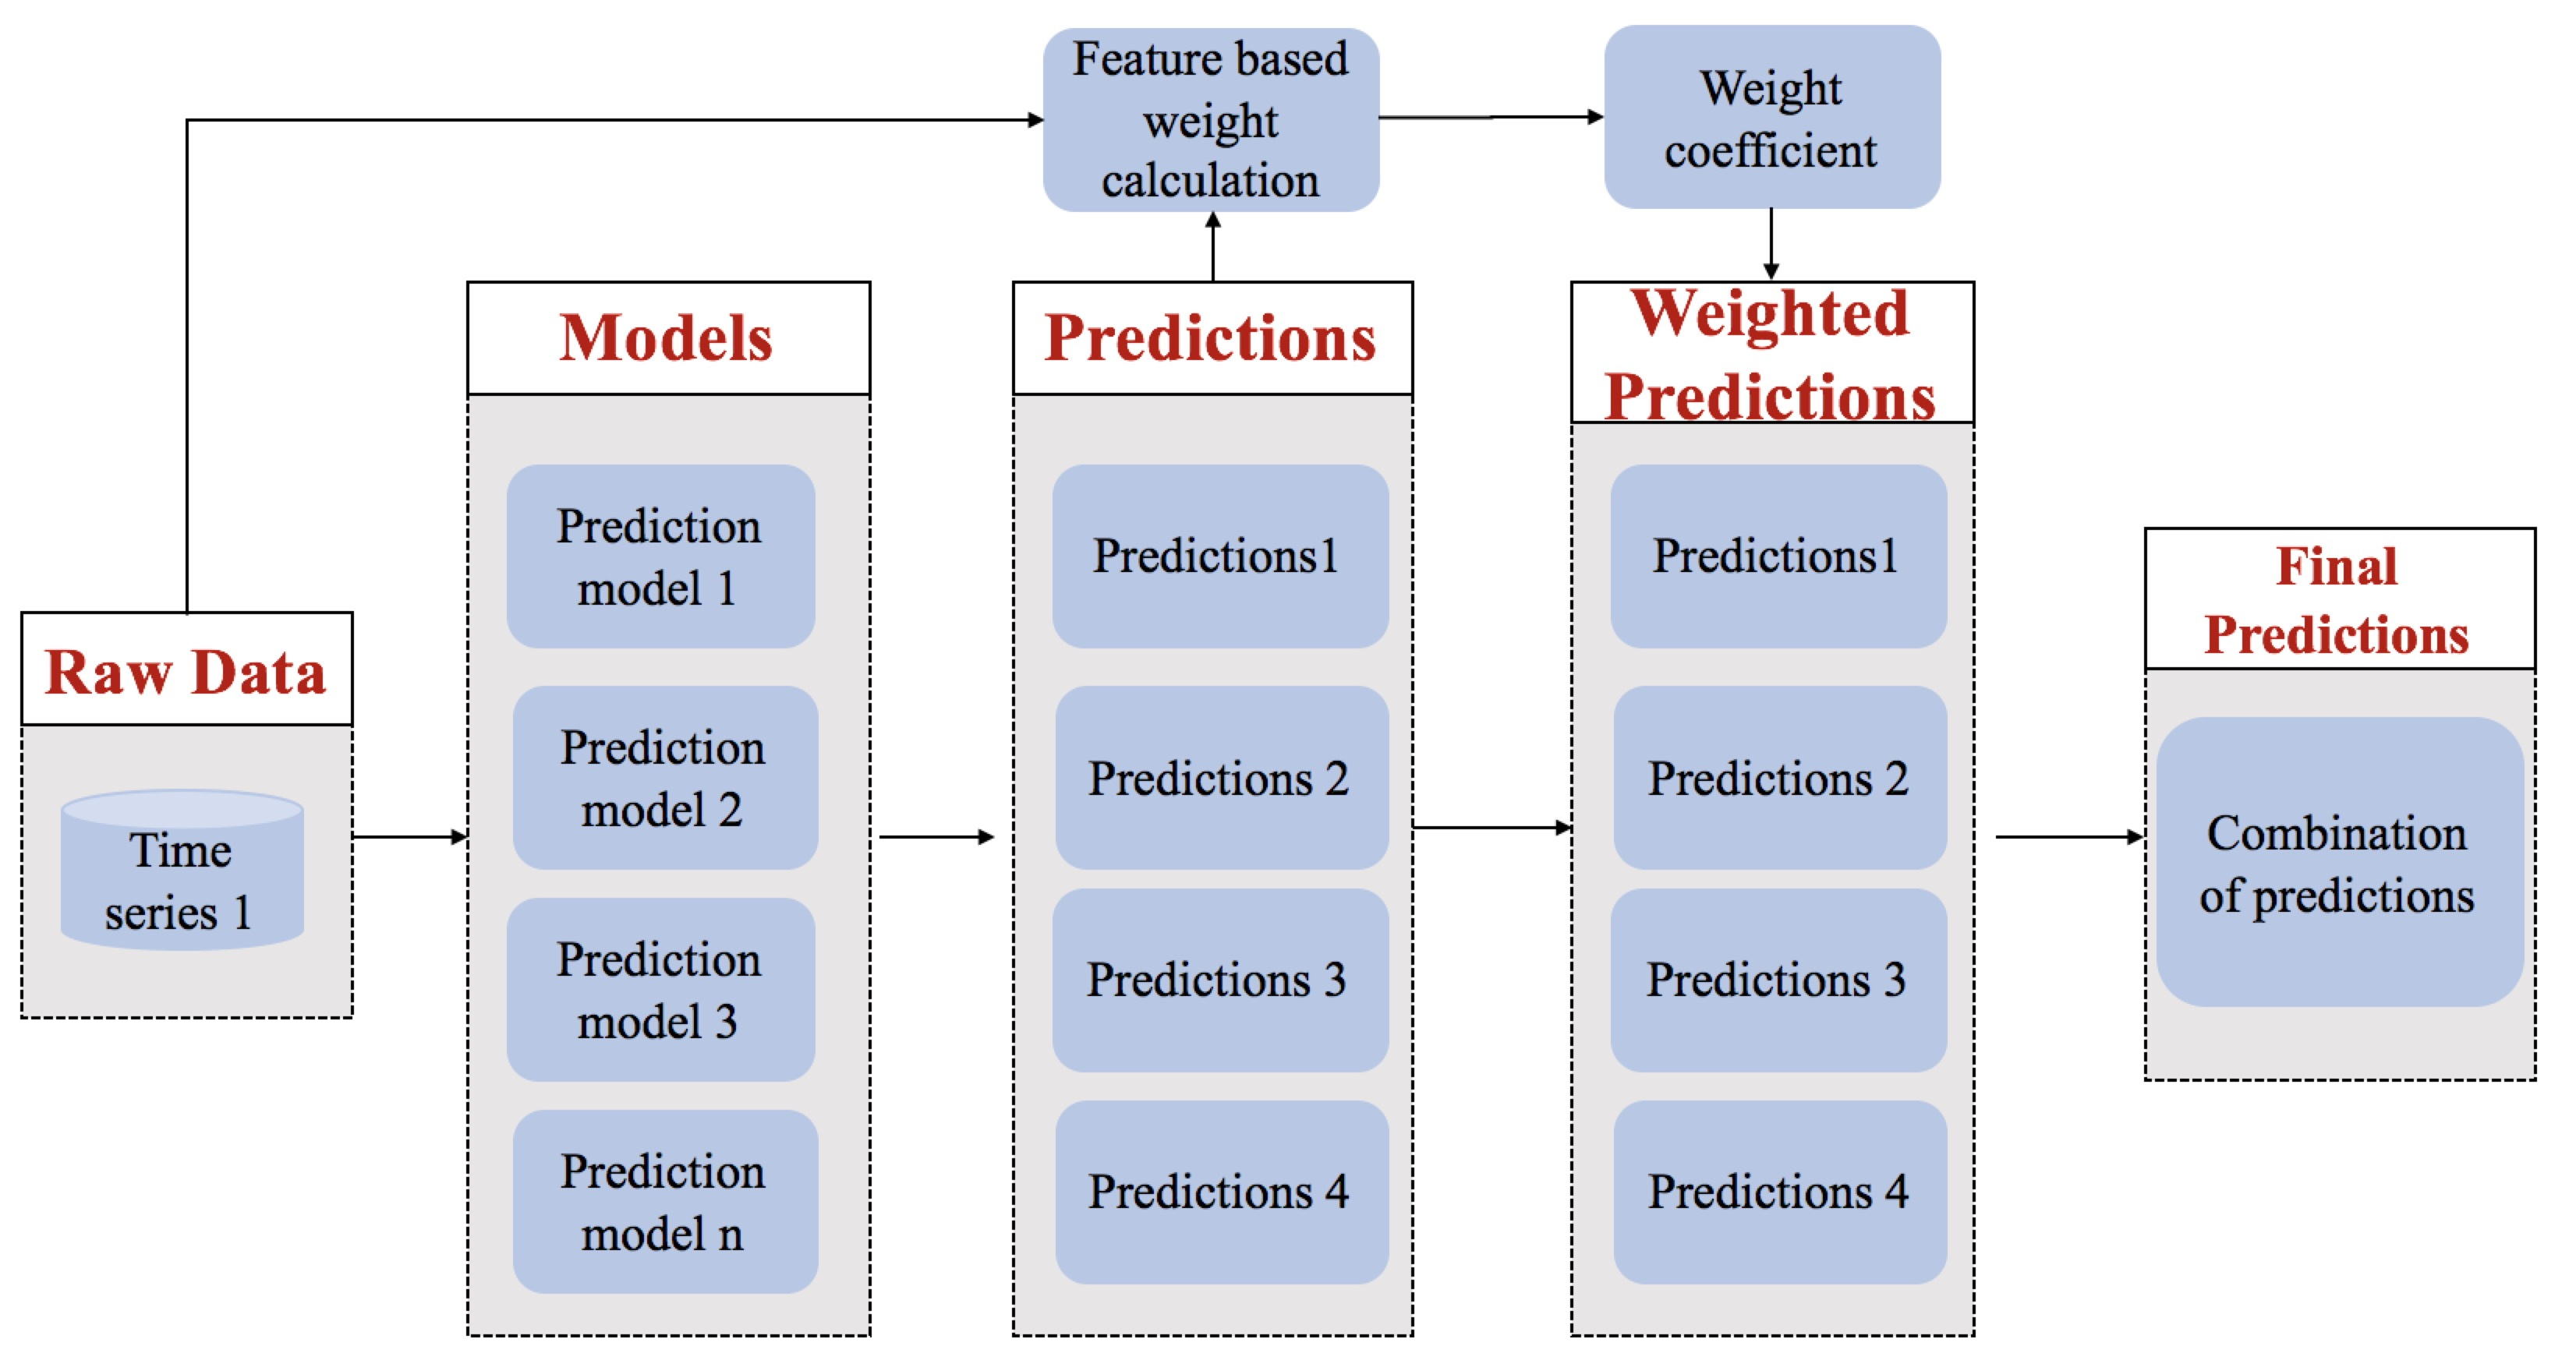
\includegraphics[width=0.7\linewidth]{figures/model-averging-feature-based}
  % \caption{Model averaging framework based on automatic feature extraction for the largest
  %   time series forecasting competition dataset.}
  \label{fig:framework}
\end{figure}

\end{frame}





\begin{frame}
  \frametitle{Model averaging}

\begin{table}
  \centering
  \resizebox{0.9\linewidth}{!}{
    \begin{tabular}{llllllll}
      \toprule
      rank        & Yearly & Quarterly & Monthly & Weekly & Daily & Hourly & Total \\
      \midrule
      \multicolumn{8}{c}{M4 competition}\\
      1 & 0.78 & 0.85 & 0.84 & 0.85 & 1.05 & 0.44 & 0.82 \\
      2 & 0.80 & 0.85 & 0.86 & 0.80 & 1.02 & 0.48 & 0.84 \\
      3 & 0.82 & 0.86 & 0.87 & 0.77 & 0.81 & 0.44 & 0.84 \\
      4 & 0.81 & 0.86 & 0.85 & 0.80 & 1.00 & 0.47 & 0.84 \\
      5 & 0.80 & 0.85 & 0.87 & 0.90 & 0.98 & 0.67 & 0.84 \\
      6 & 0.81 & 0.85 & 0.88 & 0.75 & 0.98 & 0.66 & 0.85 \\
      7 & 0.80 & 0.91 & 0.88 & 0.96 & 1.06 & 0.65 & 0.86 \\
      8 & 0.79 & 0.90 & 0.90 & 0.97 & 1.00 & 1.01 & 0.86 \\
      9 & 0.84 & 0.88 & 0.88 & 0.78 & 1.00 & 0.41 & 0.86 \\
      10 & 0.82 & 0.88 & 0.90 & 0.94 & 0.99 & 0.48 & 0.87 \\
      \midrule
      \multicolumn{8}{c}{Model averaging+Recurrence plot}\\
      $SIFT+XGBoost$ & 0.82 & 0.85 & 0.89 & 0.92 & 1.04 & 0.50 & 0.86 \\
      $\textbf{Pre trained CNN model+Classifier}$\\
      $inception-v1+XGBoost$ & 0.82 & 0.86 & 0.88 & 0.88 & 1.02 & 0.51 & 0.85 \\
      $resnet-v1-101+XGBoost$ &0.82  &0.85 &0.87  &0.88  &1.02 &0.50 &0.85     \\
      $resnet-v1-50+XGBoost$ &0.82  &0.86 &0.88  &0.87  &1.02 &0.50 &0.85     \\
      $vgg-19+XGBoost$ &0.82  &0.86 &0.88  &0.88  &1.01 &0.50 &0.85     \\
       \midrule
      \multicolumn{8}{c}{Model averaging+Gramian angular field}\\
      $\textbf{Pre trained CNN model+Classifier}$\\
       $inception-v1+Lasso$    & 0.82 & 0.86 & 0.87 & 0.86 & 1.02 & 0.51 & 0.85      \\
      $resnet-v1-101+Lasso$      & 0.82 & 0.86 & 0.88 & 0.83 & 1.03 & 0.50 & 0.85   \\
       $resnet-v1-50+Lasso$          & 0.82 & 0.85 & 0.89 & 0.84 & 1.02 & 0.50 & 0.85\\
        $vgg-19+Lasso$        & 0.82 & 0.86 & 0.88 & 0.84 & 1.02 & 0.51 & 0.86 \\
      %   $\textbf{CNN model}$\\
      % $resnet-v1-101$       &    &      &   &    &   &   &   \\
      %  $resnet-v1-50$       &    &       &   &    &   &   &    \\
      \bottomrule
    \end{tabular}
  }
\end{table}

\end{frame}

\section{Automatic time series forecasting}

\begin{frame}
  \frametitle{Automatic time series forecasting}
  \begin{itemize}
  \item Automatic time series features are extracted via machine learning (deep learning)
    algorithms.
  \item \textbf{The advantage:} The automatic extracted features are usually \textbf{not
      interpretable}.

  \item This allows for statistical forecasting when data privacy is a real concern.

  \end{itemize}

\end{frame}


\begin{frame}
  \frametitle{Automatic time series forecasting}

  \centerline{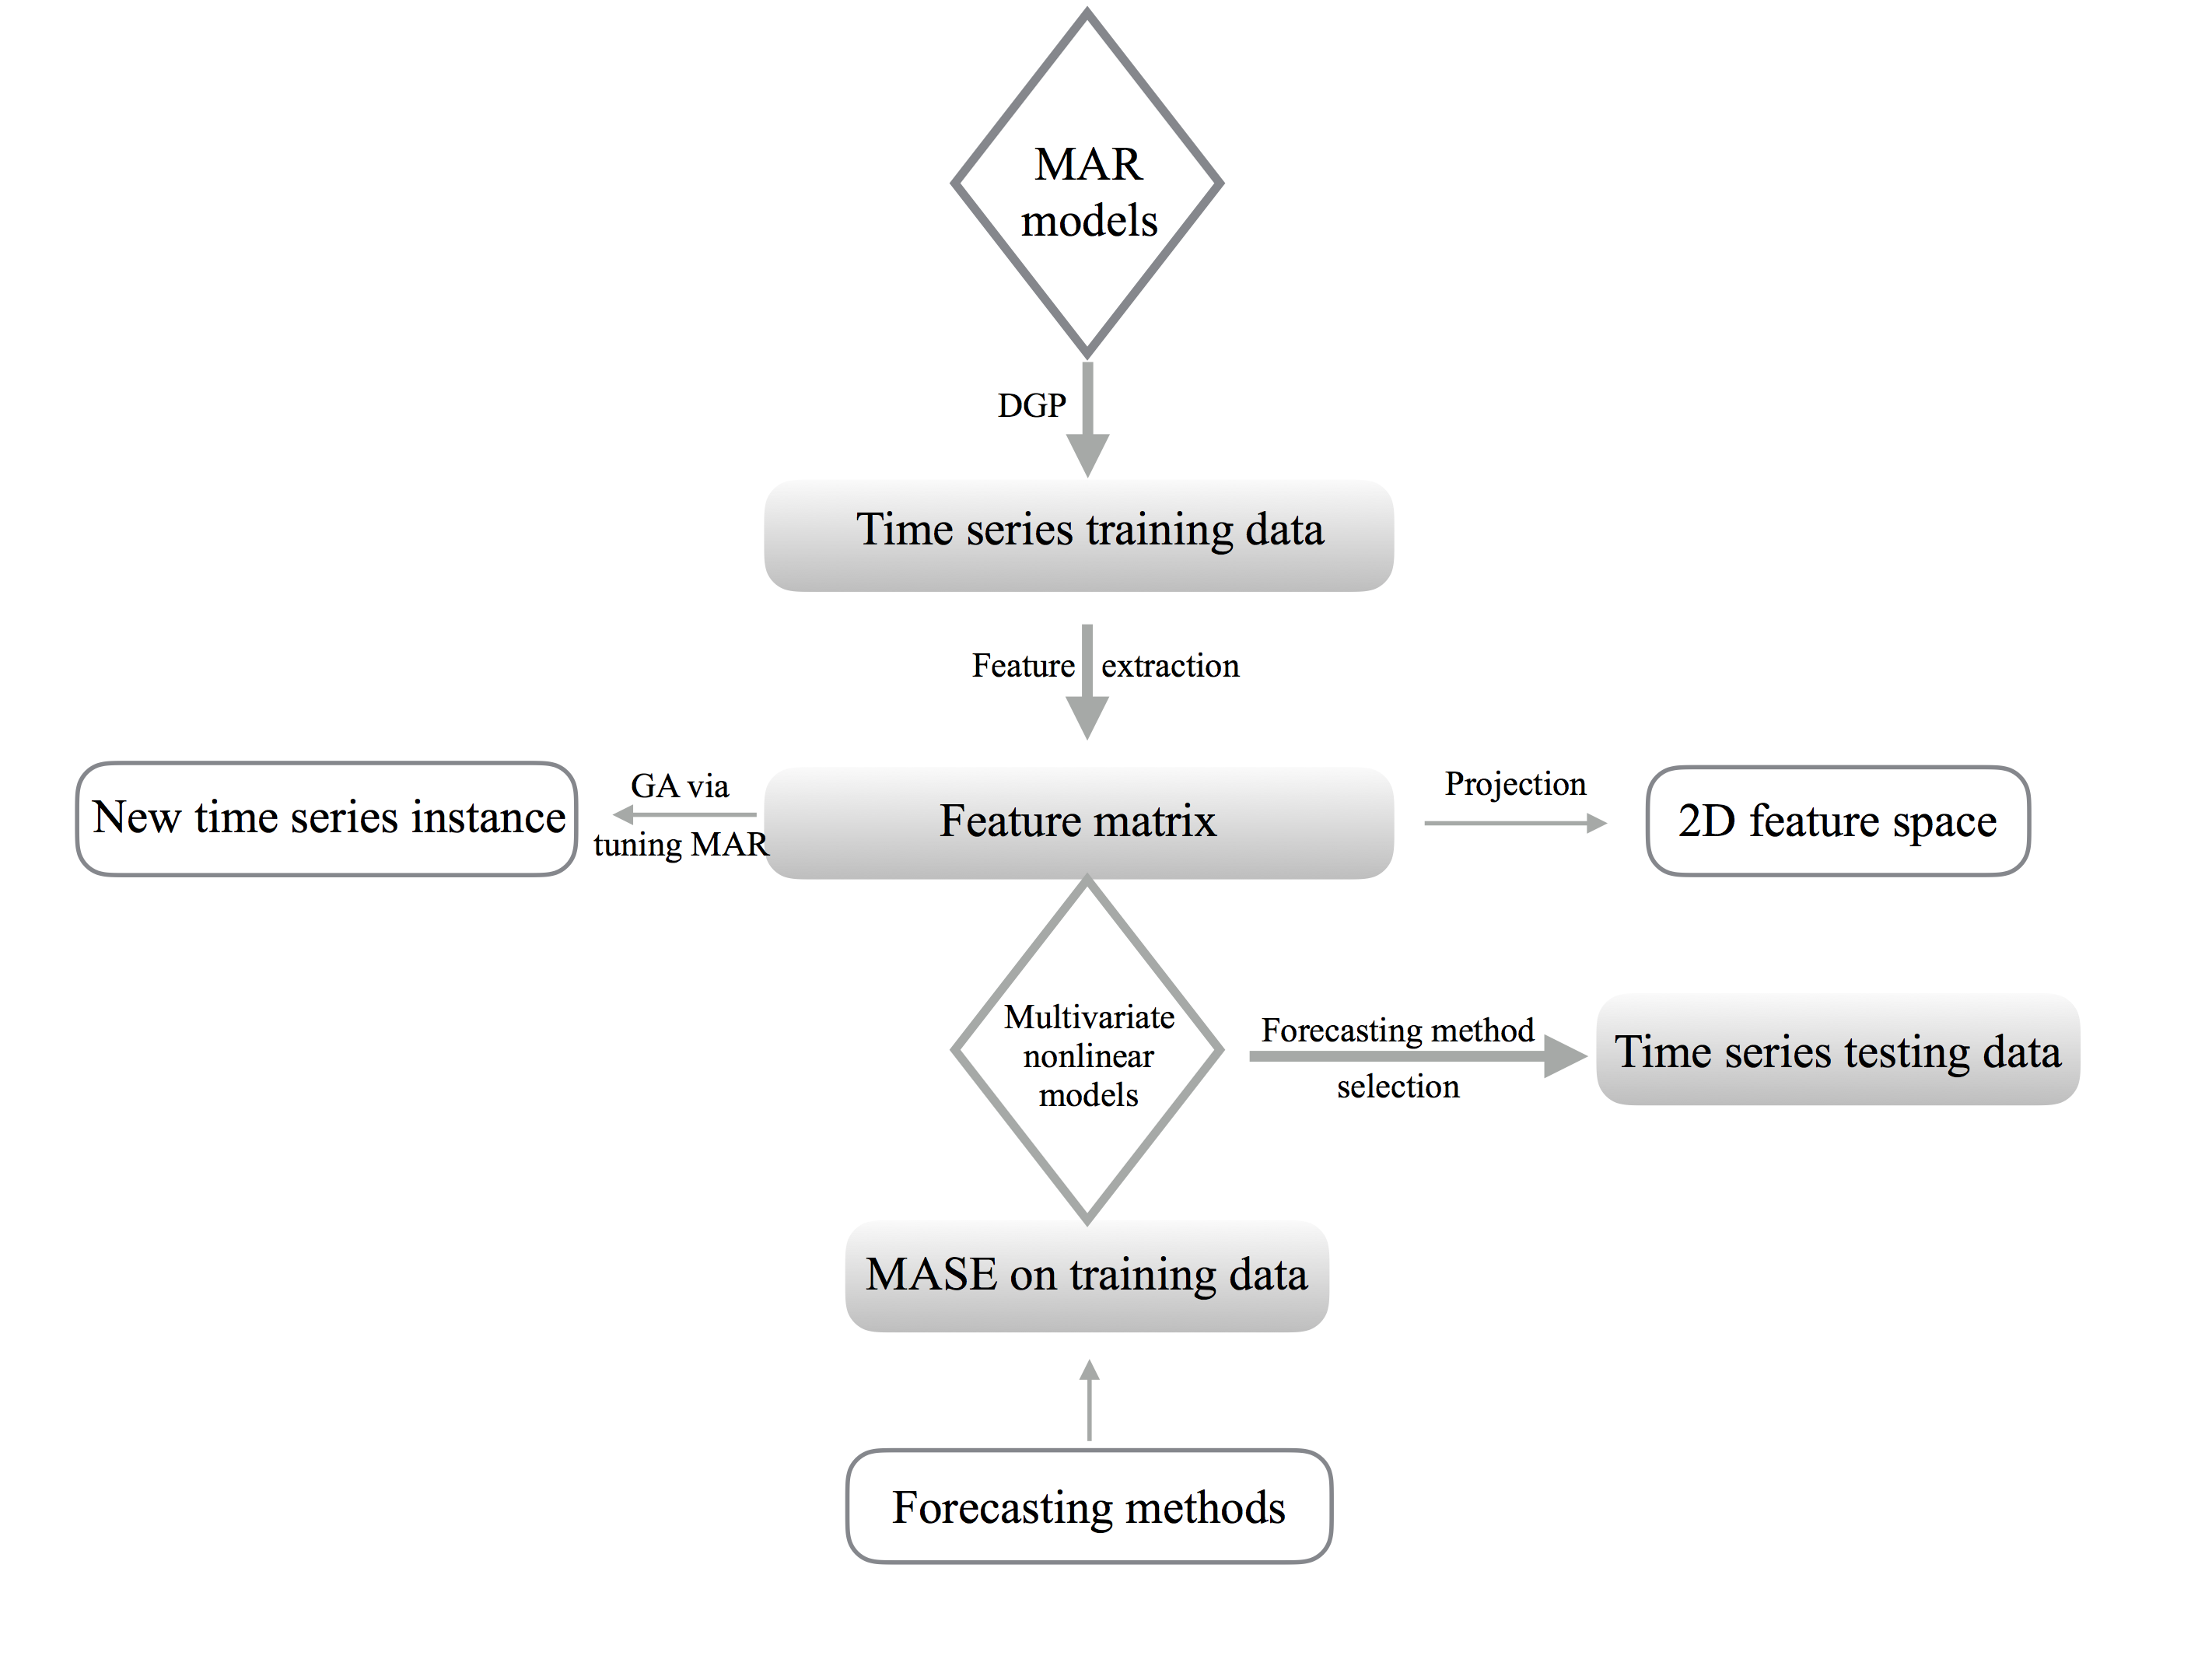
\includegraphics[height=0.6\textheight]{figures/framework.pdf}}


  \begin{itemize}
  \item Working papers for the \emph{automatic time series forecasting} framework
    \begin{itemize}
    \item   {\color{blue} Efficient generation of time series with diverse and controllable characteristics}\\
      (with Yanfei Kang and Rob Hyndman)\\
    \item {\color{blue} Forecasting using time series feature spaces}\\
      (with Yanfei Kang and Rob J. Hyndman)\\
    \item {\color{blue} Time series forecasting based on automatic feature extraction}\\
      (with Yanfei Kang,  Xixi Li)
    \end{itemize}
  \end{itemize}
\end{frame}




\begin{frame}
  \frametitle{Automatic time series forecasting}
  \framesubtitle{Automatic generated time-series-Net}
  \begin{itemize}
  \item Is ImageNet a good training source for time series image?

  \item Consist of multiple stationary or non-stationary autoregressive
    components.\\
  \item
    A \(K\)-component MAR model is defined as \citep{wong2000mixture} : \[
      F(x_t|\mathcal{F}_{t-1}) =
      \sum\limits_{k=1}^K\alpha_k\Phi(\frac{x_t-\phi_{k0}-\phi_{k1}x_{t-1}-\cdots
        -\phi_{kp_k}x_{t-p_k}}{\sigma_k}),
    \] where \(F(x_t|\mathcal{F}_{t-1})\) is the conditional cumulative
    distribution of \(x_t\) give the past information
    \(\mathcal{F}_{t-1}\). \(\Phi(\cdot)\) is the cumulative distribution
    function of the standard normal distribution.
    \(\sum_{k=1}^K \alpha_k= 1\), where \(\alpha_k > 0\),
    \(k = 1, 2, \cdots, K\).
  \end{itemize}

\end{frame}


\begin{frame}
  \frametitle{Automatic time series forecasting}
  \framesubtitle{Automatic generated time-series-Net}

  \begin{align*}
    E(x_t|\mathcal{F}_{t-1}) &= \sum\limits_{k=1}^K\alpha_k \mu_{k, t}\\
    \mathrm{var}(x_t|\mathcal{F}_{t-1}) &= \sum\limits_{k=1}^K\alpha_k \sigma_k^2 +
                                          \sum\limits_{k=1}^K\alpha_k \mu_{k, t}^2 - \left(\sum\limits_{k=1}^K\alpha_k
                                          \mu_{k, t}\right)^2.
  \end{align*}

  \begin{itemize}
  \item
    \(\mathrm{var}(x_t|\mathcal{F}_{t-1})\) changes with conditional means
    of different components.
  \item
    The shape of the conditional distributions of the time series changes
    with time.
  \item
    The MAR models can handle heteroscedasticity, which is common in
    financial time series.
  \end{itemize}

\end{frame}

\begin{frame}
    \frametitle{Automatic time series forecasting}
  \framesubtitle{Automatic generated time-series-Net}

  \begin{itemize}
  \item
    Mixtures of stationary and non-stationary components can yield a
    stationary process.
  \item
    To handle non-stationary time series, one can just include a unit root
    in each component.
  \item
    Possible to capture more (or any) time series features, since
    different specifications of finite mixtures have been shown to be able
    to approximate large nonparametric classes of conditional multivariate
    densities \citep{jiang1999on, li2010flexible, norets2010approximation}.
  \end{itemize}

\end{frame}

\begin{frame}
    \frametitle{Automatic time series forecasting}
  \framesubtitle{Automatic generated time-series-Net}

  \centerline{\includegraphics[width=\textwidth]{figures/simSettings.pdf}}

\end{frame}

\begin{frame}{Projection and visualisation in 2D space}

  \begin{block}{t-Stochastic Neighbor Embedding (t-SNE)}

    \begin{itemize}
    \item
      Main idea: convert the distances to conditional probabilities and
      minimize the mismatch (kullback-Leibler divergence) between
      probabilities before and after the mapping.

    \item Nonlinear, and retaining both local and global structure
      \citep{maaten2008visualizing,van2014accelerating}.
    \end{itemize}

  \end{block}

  \begin{block}{PCA}

    \begin{itemize}
    \item
      Linear, and putting more emphasize on keeping dissimilar data points
      far apart
    \end{itemize}

  \end{block}

\end{frame}

\begin{frame}
    \frametitle{Automatic time series forecasting}
  \framesubtitle{Automatic generated time-series-Net}


  \centerline{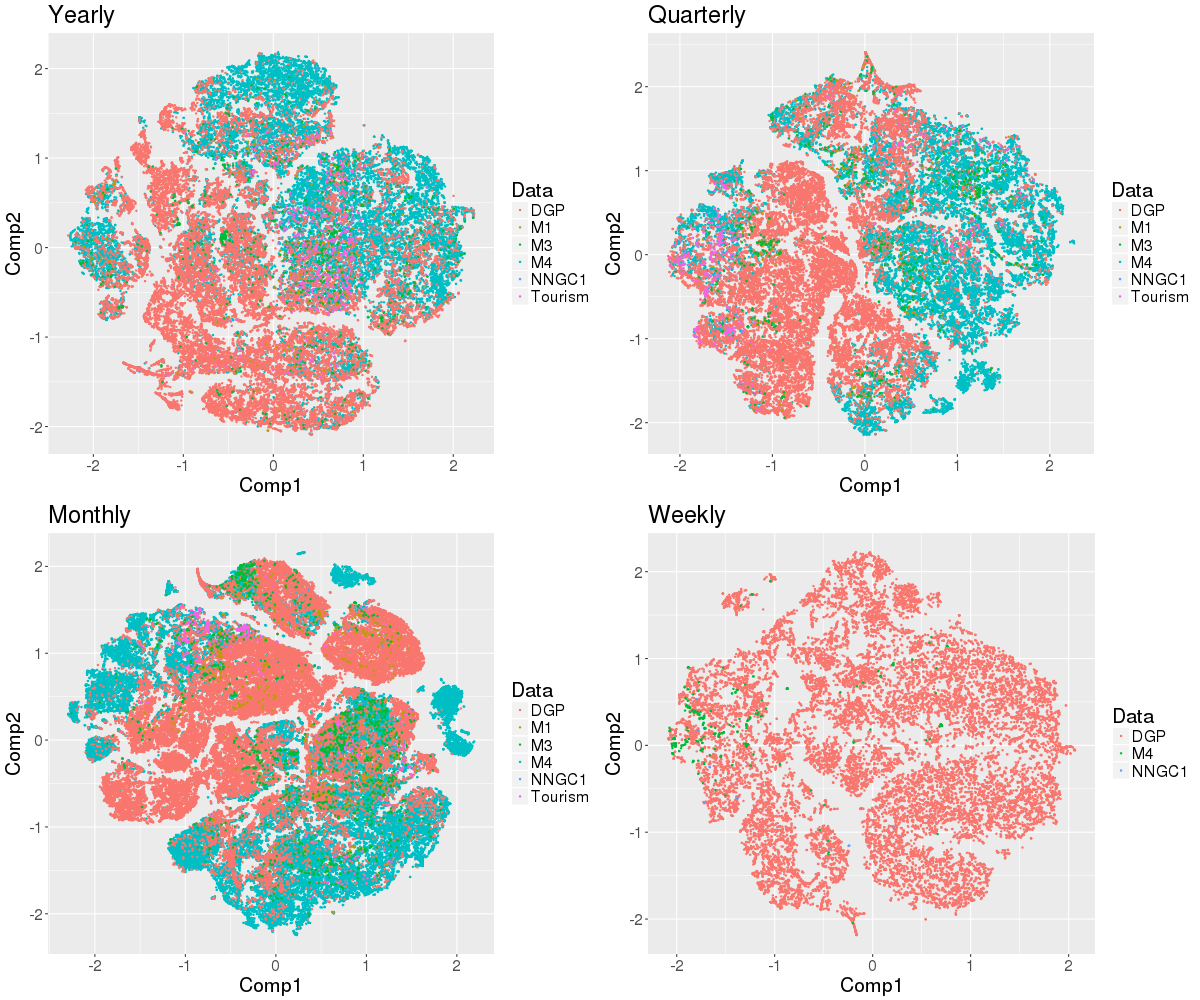
\includegraphics[width=0.8\textwidth]{figures/coverage.png}}

\end{frame}

\begin{frame}
  \frametitle{Automatic time series forecasting}
  \framesubtitle{Automatic generated time-series-Net}


  \begin{itemize}
  \item   We define the miscoverage of dataset A over dataset B as:

  \item
    Find the maximum ranges of the \(x\) and \(y\) axes reached by the two
    datasets A and B, and cut the \(x\) and \(y\) dimensions into
    \(N_b = 30\) bins.
  \item
    In the constructed two-dimensional grid with \(N_b^2 = 900\) subgrids,
    we denote \(\mathcal{I}_{i,A} = 0\) if no points in dataset A fall
    into the \(i\)th subgrid. \(\mathcal{I}_{i,A} = 1\) otherwise. The
    same defination of \(\mathcal{I}_{i,B}\) applies for dataset B.
  \item
    The miscoverage of dataset A over dataset B is defined as
    \[\text{miscoverage}_{A/B} = \frac{\sum\limits_{i = 1}^{N_b}[(1 - \mathcal{I}_{i,A})*\mathcal{I}_{i,B}]}{N_b^2}.\]
  \end{itemize}

\end{frame}

\begin{frame}
  \frametitle{Automatic time series forecasting}
  \framesubtitle{Automatic generated time-series-Net}

  \begin{table}[!thb]
    \centering
    \resizebox{0.65\textwidth}{!}{
      \begin{tabular}{p{2cm}p{1.5cm}p{1.5cm}p{1.5cm}p{1.5cm}p{1.5cm}p{1.5cm}}
        \toprule
        Dataset A & \multicolumn{6}{c}{Dataset B}\\
        \cmidrule{2-7}
                  & DGP & M4 & M3 & M1 & Tourism & NNGC1 \\
        \midrule
                  & \multicolumn{6}{c}{Yearly}\\
        DGP & 0.00 & 0.02 & 0.01 & 0.00 & 0.00 & 0.00 \\
        M4 & 0.06 & 0.00 & 0.01 & 0.00 & 0.00 & 0.00 \\
        M3 & 0.35 & 0.31 & 0.00 & 0.04 & 0.05 & 0.00 \\
        M1 & 0.55 & 0.50 & 0.25 & 0.00 & 0.09 & 0.01 \\
        Tourism & 0.51 & 0.47 & 0.22 & 0.05 & 0.00 & 0.01 \\
        NNGC1 & 0.66 & 0.61 & 0.34 & 0.13 & 0.20 & 0.00 \\
        \midrule
                  & \multicolumn{6}{c}{Quarterly}\\
        DGP & 0.00 & 0.04 & 0.01 & 0.00 & 0.00 & 0.00 \\
        M4 & 0.09 & 0.00 & 0.01 & 0.00 & 0.00 & 0.00 \\
        M3 & 0.42 & 0.34 & 0.00 & 0.04 & 0.08 & 0.01 \\
        M1 & 0.53 & 0.47 & 0.16 & 0.00 & 0.10 & 0.01 \\
        Tourism & 0.53 & 0.46 & 0.20 & 0.10 & 0.00 & 0.01 \\
        NNGC1 & 0.65 & 0.58 & 0.26 & 0.13 & 0.14 & 0.00 \\
        \midrule
                  & \multicolumn{6}{c}{Monthly}\\
        DGP & 0.00 & 0.06 & 0.00 & 0.00 & 0.00 & 0.00 \\
        M4 & 0.07 & 0.00 & 0.00 & 0.01 & 0.00 & 0.00 \\
        M3 & 0.36 & 0.32 & 0.00 & 0.06 & 0.03 & 0.00 \\
        M1 & 0.45 & 0.42 & 0.16 & 0.00 & 0.06 & 0.00 \\
        Tourism & 0.59 & 0.54 & 0.27 & 0.21 & 0.00 & 0.01 \\
        NNGC1 & 0.68 & 0.63 & 0.34 & 0.26 & 0.12 & 0.00 \\
        \midrule
                  & \multicolumn{6}{c}{Weekly}\\
        DGP & 0.00 & 0.00 &  &  &  & 0.00 \\
        M4 & 0.59 & 0.00 &  &  &  & 0.01 \\
        M3 &  &  &  &  &  &  \\
        M1 &  &  &  &  &  &  \\
        Tourism &  &  &  &  &  &  \\
        NNGC1 & 0.66 & 0.09 &  &  &  & 0.00 \\
        \bottomrule
      \end{tabular}
    }%\caption{Miscoverage of dataset A over dataset B.}
    \label{table:miscoverage}
  \end{table}



  % \centerline{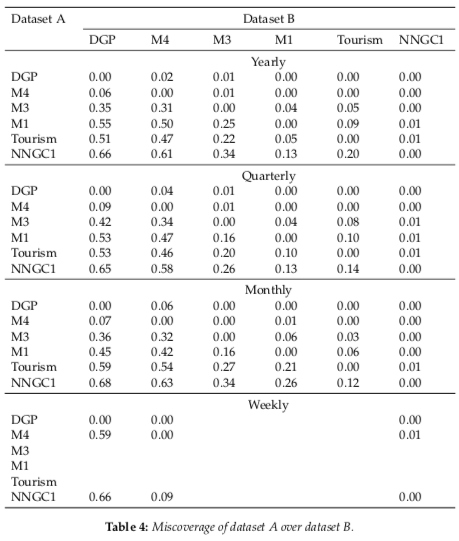
\includegraphics[height=\textheight]{figures/miscoverage.png}}

\end{frame}

\begin{frame}
  \frametitle{Ongoing work}

  \begin{itemize}
  \item Automatic density forecasting
  \item Multivariate time series forecasting
  \item Automatic forecasting for dependent time series.
  \end{itemize}

\end{frame}
\begin{frame}[plain]
  \addtocounter{framenumber}{-1}
  \begin{center}
    {\color{SUblue} \textbf{\Huge Thank you!}}
    \vspace{1cm}

    {\texttt{\textbf{\url{feng.li@cufe.edu.cn}}}}

    \vspace{1cm}

    {\texttt{\textbf{\url{http://feng.li/}}}}

  \end{center}
\end{frame}

\begin{frame}[allowframebreaks]
  \frametitle{References}
\bibliography{tsforecast-image}
\bibliographystyle{agsm}
\end{frame}

\end{document}
